% ****** Start of file apssamp.tex ******
%
%   This file is part of the APS files in the REVTeX 4.2 distribution.
%   Version 4.2a of REVTeX, December 2014
%
%   Copyright (c) 2014 The American Physical Society.
%
%   See the REVTeX 4 README file for restrictions and more information.
%
% TeX'ing this file requires that you have AMS-LaTeX 2.0 installed
% as well as the rest of the prerequisites for REVTeX 4.2
%
% See the REVTeX 4 README file
% It also requires running BibTeX. The commands are as follows:
%
%  1)  latex apssamp.tex
%  2)  bibtex apssamp
%  3)  latex apssamp.tex
%  4)  latex apssamp.tex
%
\documentclass[%
 reprint,
%superscriptaddress,
%groupedaddress,
%unsortedaddress,
%runinaddress,
%frontmatterverbose,
%preprint,
%preprintnumbers,
nofootinbib,
%nobibnotes,
%bibnotes,
 amsmath,amssymb,
 aps,
%pra,
%prb,
%rmp,
%prstab,
%prstper,
%floatfix,
]{revtex4-2}

\usepackage{graphicx}% Include figure files
\usepackage{dcolumn}% Align table columns on decimal point
\usepackage{bm}% bold math
\usepackage{hyperref}% add hypertext capabilities
\usepackage{cases}
\usepackage{subcaption}
\usepackage{subfloat}
%\usepackage[mathlines]{lineno}% Enable numbering of text and display math
%\linenumbers\relax % Commence numbering lines

%\usepackage[%showframe,%Uncomment any one of the following lines to test
%scale=0.7, marginratio={1:1, 2:3}, ignoreall,% default settings
%%text={7in,10in},centering,
%margin=1.5in,
%total={6.5in,8.75in}, top=1.2in, left=0.9in, includefoot,
%height=10in,a5paper,hmargin={3cm,0.8in},
%]{geometry}

\begin{document}

\preprint{APS/123-QED}

\title{Predicting Default on Credit Card Debt using Logistic Regression and Neural Networks}% Force line breaks with \\
% \thanks{A footnote to the article title}%

\author{Christer Dreierstad, Hans Erlend Bakken Glad}
 %Lines break automatically or can be forced with \\
\author{Torbjørn Lode Gjerberg}
\altaffiliation{Institute of Informatics, University of Oslo}
\author{Stig-Nicolai Foyn}
\altaffiliation{Institute of Geoscience, University of Oslo}
\affiliation{Institute of Physics, University of Oslo}


\date{\today}

\begin{abstract}
In this paper we discuss using logistic regression and neural networks for classification on the Taiwan credit card data. Due to the clear bias in our dataset we use different metrics to quantify the quality of our model. In particular we found that area under curve (AUC) would be a better measure of the model quality. We observe that neural networks are slightly better at classifying large and complex datasets than logistic regression. In the case of the credit card data we got $AUC = 0.76$ for logistic regression and $AUC = 0.77$ for neural networks.

In addition we compare the use of neural networks to ordinary least squares, Ridge regression and Lasso regression on the Franke function without noise. We found that using high polynomial degrees would lead to the classical regression methods outperforming our neural network. Ridge was found in our previous paper to be more resistant to overfitting and would therefore perform better on many regression problems. The best score we got with Ridge was $R^2 = 0.9999$ while with neural networks we got $R^2 = 0.9974$, both can be considered reasonably good scores. This leads to us concluding that neural networks are quite well suited for many different problems and will often have results comparable or even better than other methods.
\end{abstract}

%\keywords{Computational Science, Regression Methods: Ordinary Least Squares, Ridge, Lasso}%Use showkeys class option if keyword
\maketitle

%\tableofcontents

\section{Introduction\label{sec:intro}}
Machine learning is an emerging field in computational science. In particular, neural networks have seen an upswing in popularity due to the increase in computational power. The general idea behind a neural network is not new, but the potentially high cost in compute cycles (particularly for deep neural networks) made their implementation unfeasible in the past. Neural networks can be used for both classification and regression problems.

In this paper, our main goal is to use a feed forward neural network (FFNN) and logistic regression for classification. The two methods are built from scratch using Python, and their performance is then compared to pre-made functions from the scikit-learn library. We will consider a dataset containing user information of credit card costumers from Taiwan, courtesy of the University of California, Irvine \cite{creditcard}. This data is used to predict whether or not someone defaults on their credit card payment, given information about the costumers (marital status, sex, education etc.) and their previous payment(s).

To assess the versatility of neural networks we will also use it for regression on the Franke function. The performance of the neural network is then compared to the results from using ordinary least squares, ridge regression and lasso regression as was presented in our previous paper.


\section{Data}
\begin{figure*}[t]
\includegraphics[width=2\columnwidth]{corr_matrix.pdf}
\caption{\label{fig:corr_matrix} Correlation matrix of the default of credit card clients dataset. Last row/column states DefaultPaymentNextMonth.}
\end{figure*}

\subsection{Default of Credit Card Clients}
The dataset contains credit card usage and payment information and some information about the details of 30000 customers, as well as whether or not they defaulted on the payment. The aim is to classify credit card customers in two groups depending on whether they defaulted on payment based on the 23 explanatory parameters, mentioned initially.

We remove the samples where the features concerning the billing amount and payment amount are 0, since this represents samples where the costumer has not used their credit card.

Looking at Fig. \ref{fig:corr_matrix} showing the correlation matrix for the credit card data we find strong correlations between the groups of the different payment amounts and repayment respectively. The correlation matrix also shows that the group of explanatory variables representing repayment over previous months have the highest correlation with the default next month.

Several of the predictors in the dataset are split into multiple different independent categories, we therefore need to encode the categorical predictors such that all the predictors will be treated equally when attempting to classify the probability of defaulting. We will be using a one-hot encoder from from the scikit-learn library to transform every feature into one-hot encoded features. One-hot encoding is splitting the data into a vector consisting of zeros and ones where the position of the number 1 represents the category. E.g. the marital status of a client can be single = 1, married = 2 or other = 3. This will be categorized with a one-hot encoder as vectors $(1,0,0)$, $(0,1,0)$ and $(0,0,1)$ which is married, single and other respectively. The end result of this encoding is that the matrix of datapoints will be expanded from having 23 predictors (features) to having 89. This results in a matrix of datapoints on which we can use our classification methods. The data is also scaled using scikit-learn's StandardScaler. The StandardScaler scales each feature by subtracting its mean and dividing by the standard deviation.

\subsection{Franke Function}\label{sec:franke_data}
Artificial data is generated using the Franke function:
%
\begin{align*}
f(x,y) = &\frac{3}{4} \exp\left( -\frac{(9x-2)^2}{4} -\frac{(9y - 2)^2}{4} \right) \\+&\frac{3}{4} \exp\left( -\frac{(9x+1)^2}{49} - \frac{(9y + 1)^2}{10} \right) \\+&\frac{1}{2} \exp\left( -\frac{(9x-7)^2}{4} - \frac{(9y - 3)^2}{4} \right)\\-&\frac{1}{5} \exp\left( -(9x-4)^2 - (9y - 7)^2 \right) .
\end{align*}
%
Here, $x$ and $y$ can be seen as the coordinates of some area. The "height" $z$ is then generated using this function, so that
%
\begin{equation}
z(x, y) = f(x, y) .
\end{equation}
%
Using the Franke function to produce values over some domain (in our case, $x, y \in [0,1]$), we get a dataset to perform predictions on using a neural network. The performance is then compared using ordinary least squares, ridge regression and lasso regression.

\begin{figure}[h!]
\includegraphics[width=\columnwidth]{rocheatmap_20e_100b_64_32_16_sigsigsigsig.pdf}
\caption{\label{fig:roc_heatmap_NN_CC} ROC area under curve scores for neural network on credit card default data. 50 epochs, 100 mini batch size, three hidden layers of 64, 32 and 16 neurons. Sigmoid activation functions for hidden and output layers.}
\end{figure}

\begin{figure}[h!]
\includegraphics[width=\columnwidth]{testacc_20e_100b_64_32_16_sigsigsigsig.pdf}
\caption{\label{fig:test_acc_NN_CC} Test accuracy for neural network on credit card default data. 50 epochs, 100 mini batch size, three hidden layers of 64, 32 and 16 neurons. Sigmoid activation functions for hidden and output layers.}
\end{figure}

\begin{figure}[h!]
\subfloat{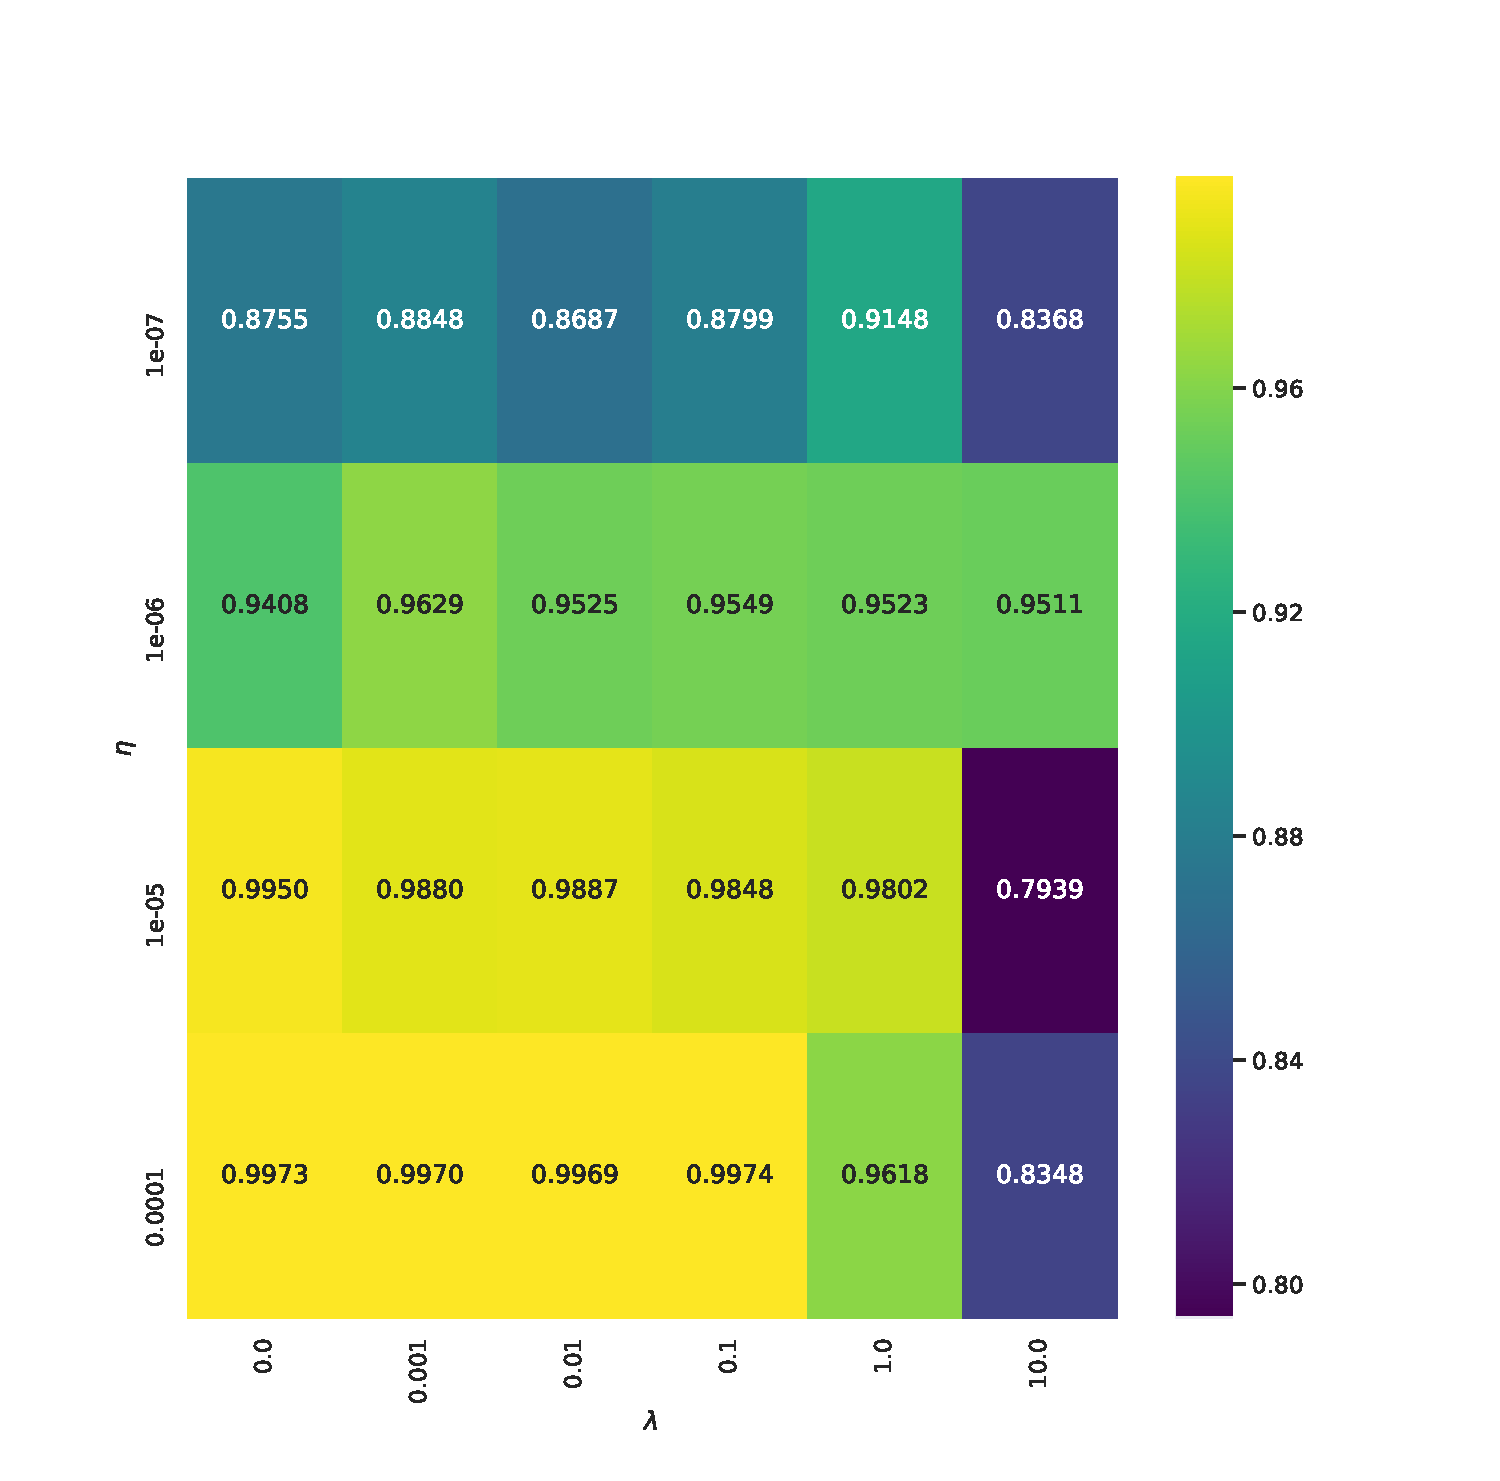
\includegraphics[clip,width=\columnwidth]{r2_FF_50e_100b_100_50_tanhtanh.pdf}
  \subcaption{R2 score}}
\subfloat{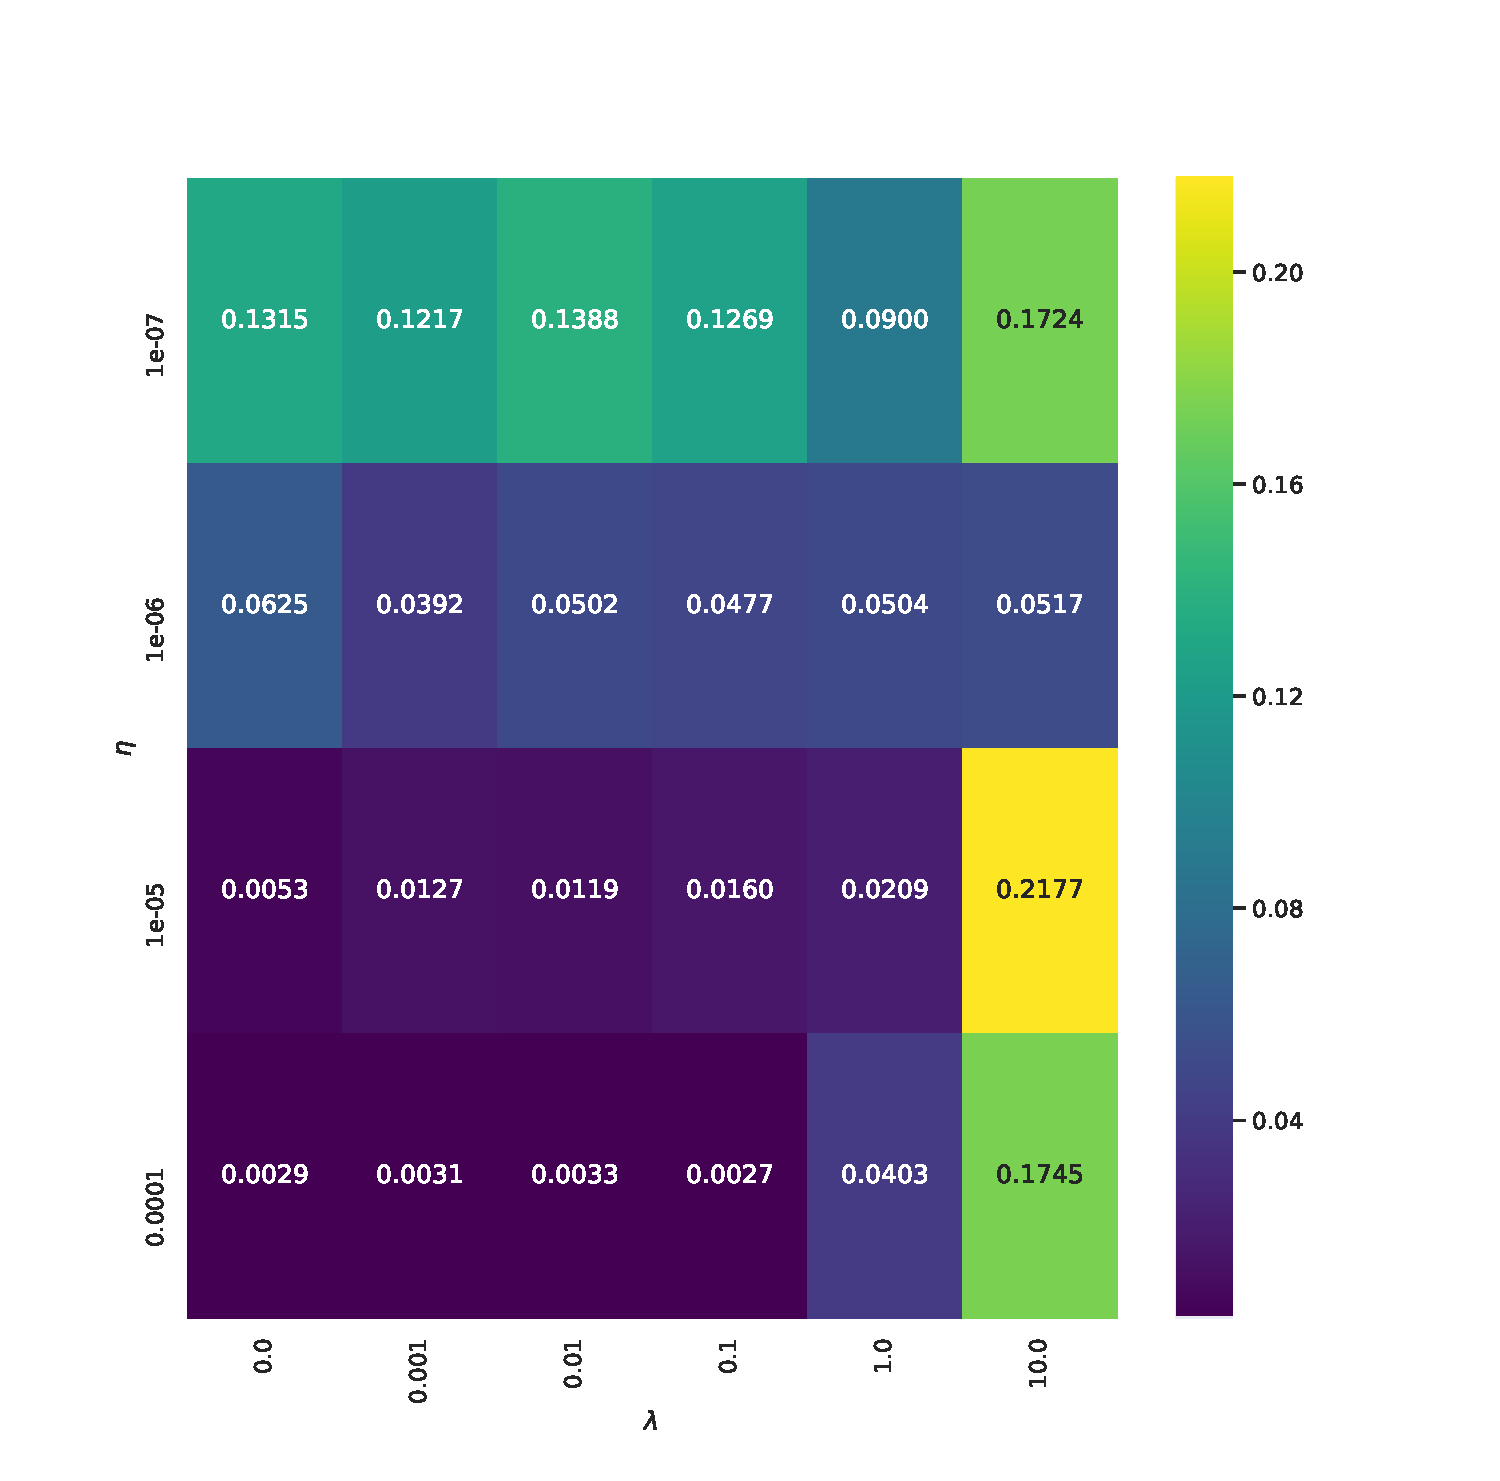
\includegraphics[clip,width=\columnwidth]{mse_FF_50e_100b_100_50_tanhtanh.pdf}
  \subcaption{MSE}}
\caption{Heatmap of MSE and R2 for the Franke function using neural network. Varying learning rate $\eta$ and penalty $\lambda$. Two hidden layers with 100 and 50 neurons, 50 epochs and a batch size of 100. Activation functions used in hidden layers are both the hyperbolic tangent.}
\label{fig:mse_r2_NN}
\end{figure}

\section{Methods}\label{sec:methods}

\subsection{Gradient Descent}\label{sec:gradient_descent}
Gradient descent (GD) is used to locate minima of a function, with aim of locating the global minima. GD is an important optimization tool used in several different machine learning algorithms. In a NN GD is used to update the weights and biases until convergence.

The simplest GD method is similar to Newton's method for finding minima by extending tangent from the current point. By calculating the negative gradient at a point on the curve, choosing a step length (constant, else steepest descent method),  GD will by iterations move towards a minima. We can see this by
%
\begin{equation}
    x_{k+1} = x_{k} - \gamma_{k}\nabla F(x_k),
\end{equation}
%
where $\gamma_k$ represents step length and $\nabla F(x_k)$ is the largest gradient in the step $x_k$. In neural
networks $\gamma_k$ is typically called the learning rate. If $\gamma_k > 0$ and small enough then $F(x_{k+1}) \leq F(x_k)$ and the system moves towards a minima. In general it is impossible to know if GD finds the global or local minima unless dealing with a convex function. How fast GD converges is highly dependant upon the initial choice of where to start calculating from. The regular gradient descent has a risk of finding a local minima, possibly giving a poor result.

A different gradient descent method is Stochastic Gradient Descent (SDG) with mini-batches. SGD relies on the idea that the cost function can be written as a sum over the data points
%
\begin{equation}
    C(\beta) = \sum_{i}^{n} c_i(\boldsymbol{x_i}, \beta).
\end{equation}
%
For each mini batch the data points are chosen at random. The gradient of each mini-batch is computed separately with different starting points and will likely find different local minima. The gradient of the cost function is computed as the sum over the gradient of each batch as
%
\begin{equation}
    \nabla_{\beta} C(\beta) = \sum_{i=1}^{n} \nabla c_i(\boldsymbol{x_i}, \beta)
\end{equation}
%
 in a similar manner to the cost function itself. This SGD method is not reliant on initial values to produce good results.

\subsection{Classification}
For the credit card dataset we will consider two classifiers; logistic regression and FFNN.

\begin{figure}[h!]
\subfloat{
  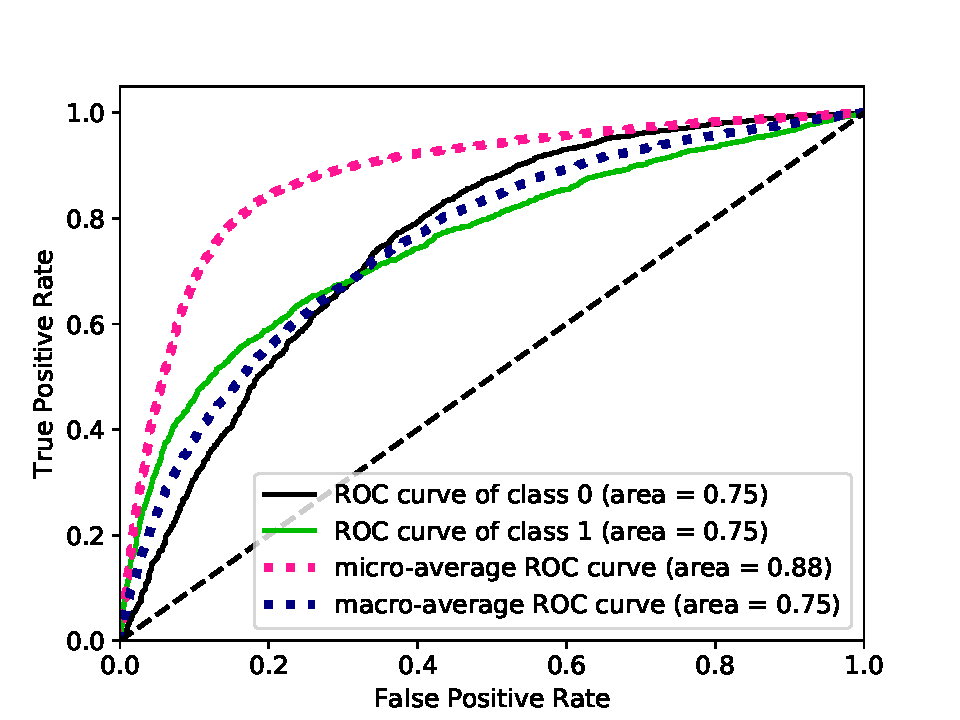
\includegraphics[clip,width=\columnwidth]{ROC_Logreg_50e_100b_GD.pdf}
  \subcaption{Gradient descent with 10000 iterations.}
}
\subfloat{
  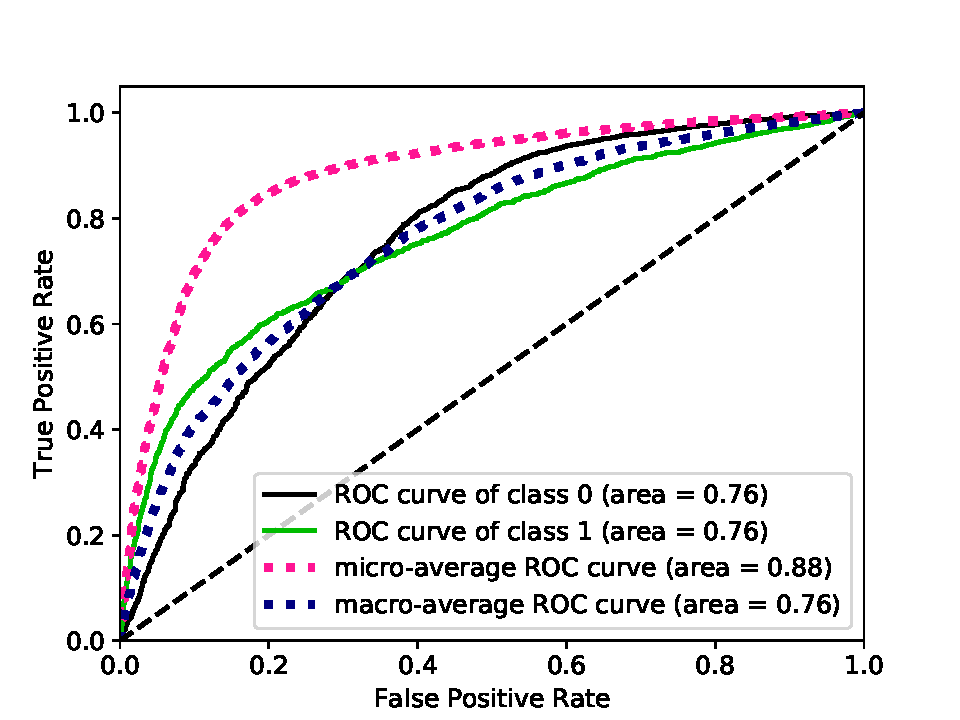
\includegraphics[clip,width=\columnwidth]{ROC_Logreg_50e_100b_SGD.pdf}
  \subcaption{Stochastic gradient descent.}
}
\subfloat{
  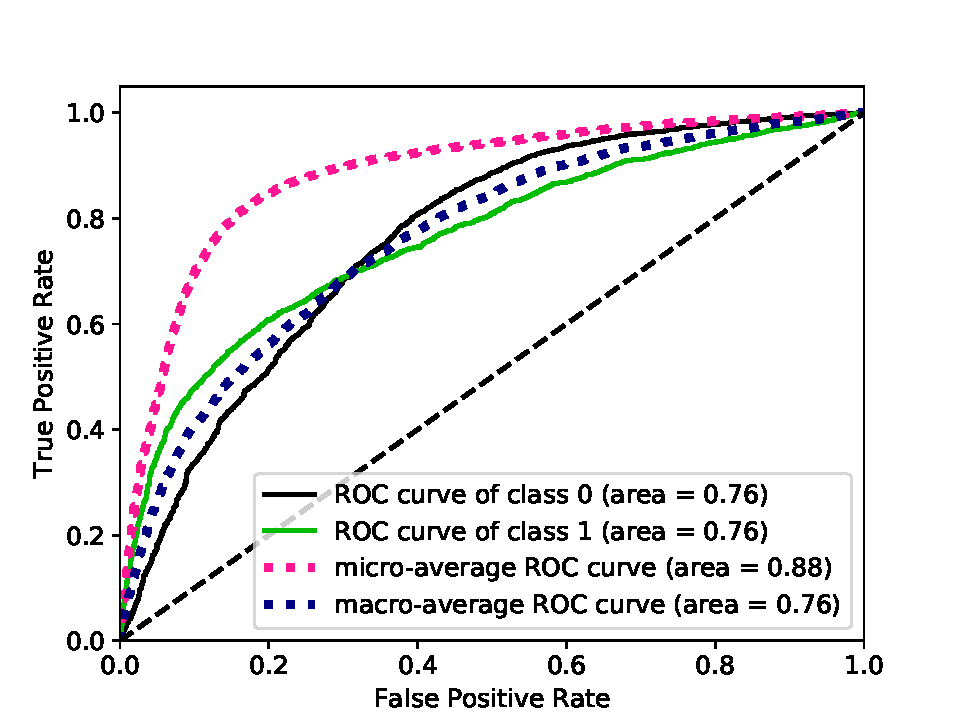
\includegraphics[clip,width=\columnwidth]{ROC_Logreg_50e_100b_Sklearn.pdf}
  \subcaption{Scikit-learn.}
}
\caption{ROC curves for credit card default data using logistic regression.}
\label{fig:roc_curves_logreg}
\end{figure}


\subsubsection{Logistic Regression}
The goal of logistic regression is to classify a given input into an appropriate category. In this paper we will only consider binary logistic regression, i. e. we only have two possible categories (default or no default on credit card debt).

Given some data $\boldsymbol{X}$ with dimensions $(n_{\textrm{samples}}, m_{\textrm{features}}+1)$, we want to determine the classifications $\boldsymbol{y}$ of the given samples. The additional column in the design matrix $\boldsymbol{X}$ represents the intercept. In the binary case, the possible classifications are $y_i = 1$ (pass) and $y_i = 0$ (fail). We assume that the features can be assigned weights $\boldsymbol{\beta}$ as in the linear regression case, where we assume a model
%
\begin{equation*}
\boldsymbol{y} = \boldsymbol{X}\boldsymbol{\beta} + \boldsymbol{\epsilon},
\end{equation*}
%
with normally distributed noise $\boldsymbol{\epsilon}$. We will use $y$ for the real values of the dependent variable and $\hat{y}$ for the estimated value.

The issue with using a plain linear model such as this is that the outputs are continuous values, while our goal is to categorize the samples, i. e. determining if $\hat{y_i} = 0$ or $\hat{y_i} = 1$. In logistic regression, we make use of the logistic function (also called sigmoid):
%
\begin{equation}\label{eq:sigmoid}
p(t) = \frac{1}{1 + e^{-t}} .
\end{equation}
%
For an input $t$, this function outputs the likelihood of some given event. With binary logistic regression, the input is the predicted values from linear regression and the possible events are either pass or fail. For a single data point $x_i$ with $m$ features the probability of getting $\hat{y_i} = 1$ (pass) is then
%
\begin{equation*}
p(\hat{y_i} = 1 \ | \ x_i, \boldsymbol{\beta}) = \frac{1}{1 + e^{-x_i\boldsymbol{\beta}}},
\end{equation*}
%
and the probability for $\hat{y_i} = 0$ (fail) is simply
%
\begin{equation*}
p(\hat{y_i} = 0 \ | \ x_i, \boldsymbol{\beta}) = 1 - p(\hat{y_i} = 1 \ | \ x_i, \boldsymbol{\beta}) .
\end{equation*}
%
In other words, passing $x_i\boldsymbol{\beta}$ through the sigmoid gives the probability of sample $x_i$ taking the value $\hat{y_i} = 1$. We then determine the predicted category by checking whether or not the probability exceeds a certain threshold, typically set to 0.5:
%
\begin{equation*}
\hat{y_i} =
\begin{cases}
1 \ \textrm{if} \ p(x_i\boldsymbol{\beta}) \geq 0.5 \\
0 \ \textrm{if} \ p(x_i\boldsymbol{\beta}) < 0.5
\end{cases}
\end{equation*}

\begin{figure}[h!]
\subfloat{
  \includegraphics[clip,width=\columnwidth]{roc_20e_100b_64_32_16_sigsigsigsig.pdf}
  \subcaption{Own NN with 50 epochs and batch size 100.}
}
\subfloat{
  \includegraphics[clip,width=\columnwidth]{roc_64_32_16_NNskl_sig.pdf}
  \subcaption{Sklearn MLPClassifier neural network.}
}
\caption{ROC AUC curves on credit card data. Neural network has three hidden layers with 64, 32 and 16 neurons. Sigmoid activation function.}
\label{fig:roc_curves_NN}
\end{figure}

%
The estimates $\boldsymbol{\hat{y}}$ can then be compared to the true values $\boldsymbol{y}$ as a performance metric. In classification, the accuracy score of a model tested on $n$ samples is defined as
%
\begin{equation*}
\textrm{Accuracy} = \frac{\sum_{i}^n I(y_i = \hat{y_i})}{n} ,
\end{equation*}
%
and represents the fraction of samples that are classified correctly. The indicator function $I$ is equal to 1 when the condition is fulfilled, and 0 otherwise.

With logistic regression, $\boldsymbol{\beta}$ is typically initialized with random values. The parameters are then optimized as explained in the next section.

\subsubsection{Finding Optimal Parameters}
The ideal values of $\boldsymbol{\beta}$ (the parameters that give the best accuracy score) are not immediately known. For this purpose, we define a cost function $C(\boldsymbol{\beta})$. This function gives us an estimate of the error that our model makes when attempting to classify a sample. For this problem we choose the \textit{cross-entropy} as our cost function,
%
\begin{equation*}
    C(\boldsymbol{\beta}) = -\sum_{i=1}^n \left( y_i(x_i\boldsymbol{\beta} - \log(1 + \exp(x_i\boldsymbol{\beta}\right) .
\end{equation*}
%

The optimal values for our parameters are then determined by which values of $\boldsymbol{\beta}$ that minimize the cost. Thus we need the derivative of the cost function w. r. t. the parameters, which is
%
\begin{equation*}
    \frac{\partial C(\boldsymbol{\beta})}{\partial \boldsymbol{\beta}} = \boldsymbol{X}^T(\boldsymbol{p} - \boldsymbol{y}) .
\end{equation*}
%
Ideally we want $\partial C / \partial \boldsymbol{\beta} = 0$, but since we are dealing with a multi-dimensional problem (multiple features per sample) the global minimum of the cost function is not easily found. One method of finding an approximate global minimum is through gradient descent, which we will be using as explained in section \ref{sec:gradient_descent}.


\subsubsection{Multilayer Perceptron}
A feed forward neural network is the simplest type of artificial neural network. In this type of neural net the information can only go from input to output. A multilayer perceptron is a type of feed forward neural network that consists of an input layer, one or more hidden layers and an output layer.

Each neuron will have weights and biases that dictate their influence on the neurons in the next layer. The biases restrict the minimum weight needed for a neuron to have an effect on the next layer. Information is processed through the different layers by going through each layers activation function. Eventually we will get an output which usually will just be a random guess. For the network's results to improve we use gradient decent on the cost function of the network. This will let the network adjust its weights and biases through backward propagation. We repeat the process, assuming that the results improve for each cycle and eventually we can test our final model.

\begin{figure}[h!]
\subfloat{
  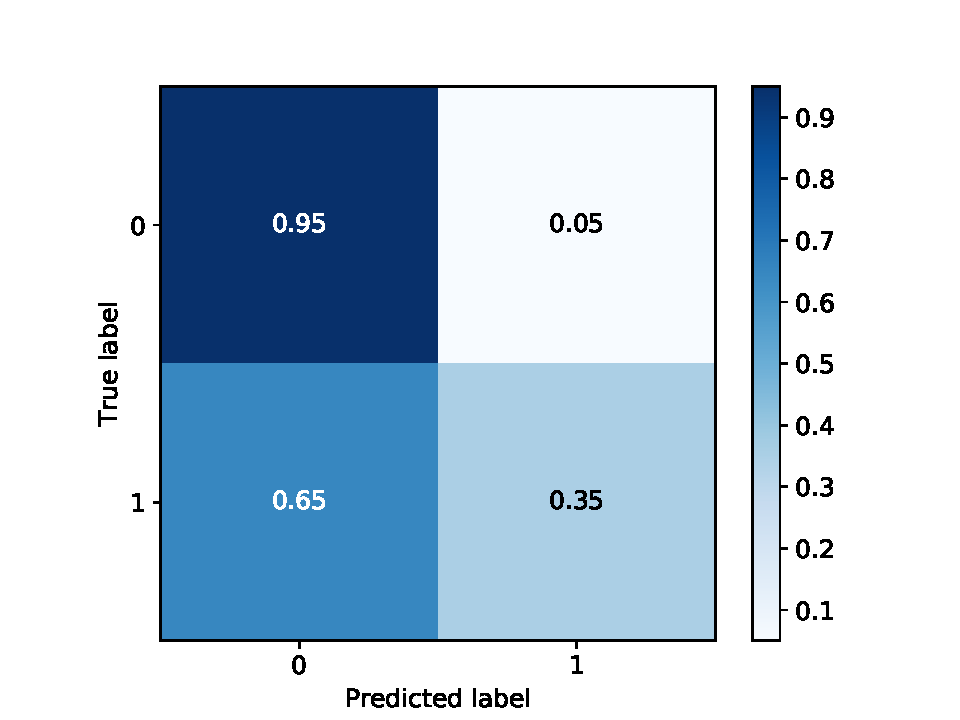
\includegraphics[clip,width=\columnwidth]{conf_Logreg_50e_100b_GD.pdf}
  \subcaption{Gradient descent with 10000 iterations.}
}
\subfloat{
  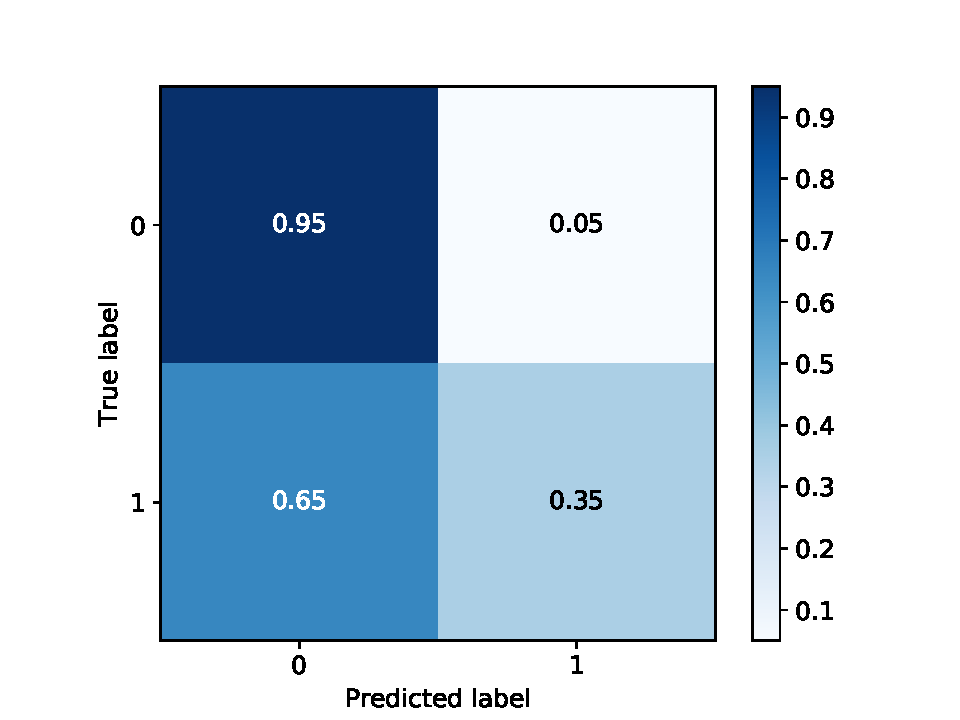
\includegraphics[clip,width=\columnwidth]{conf_Logreg_50e_100b_SGD.pdf}
  \subcaption{Stochastic gradient descent. }
}
\subfloat{
  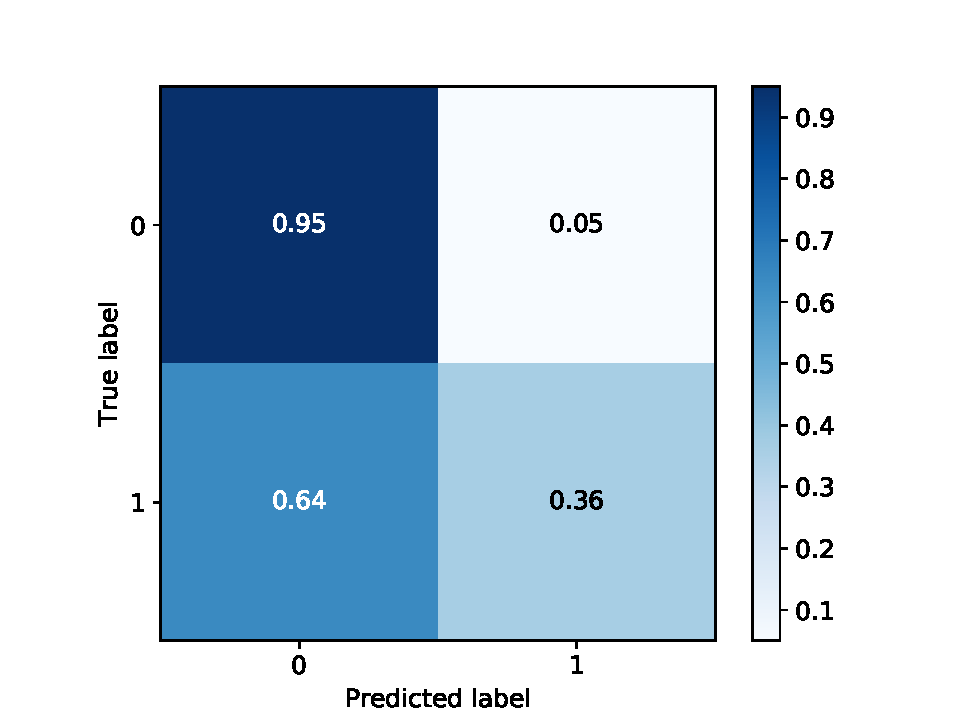
\includegraphics[clip,width=\columnwidth]{conf_Logreg_50e_100b_Sklearn.pdf}
  \subcaption{Scikit-learn.}
}
\caption{Normalized confusion matrices on credit card default data using different types of logistic regression.}
\label{fig:conf_matrices_logreg}
\end{figure}

Each layer of a multilayer perceptron has an activation function that takes a weighted sum $z_i^l$. The sum is given by $z_i^l = \sum_{j=1}^{M} w_ {ij}^l x_j + b_i^l$ in the input layer and $z_i^l = \sum_{j=1}^{M} w_ {ij}^l a_j^{l-1} + b_i^l$ in the layers after. Here $a_j^l = f(z_j^l)$ which is the activation function that contributes to the weighted sum of all the layers after. All neurons in a layer use the same activation function, but there can be different functions from layer to layer. Computing these weighted sums for each layers, with the previous layer affecting the next, is called a feed forward pass.

The activation functions in a multilayer perceptron neural network are subject to a set of restrictions to fulfill the universal approximation theorem. It must be non-constant, bounded, monotonically increasing  and continuous. This excludes linear functions as they are not bounded. With a linear function the neural network would also, regardless of complexity, be a linear transformation. The non-linear functions used in the neural network were sigmoid (Eq. \eqref{eq:sigmoid}) and hyperbolic tangent, where the latter is used for the case of regression on the Franke function.

After a feed forward pass we will receive a result that will get a correction from our gradient decent algorithm. This is where we use back propagation to correct all the weights and biases throughout our network. The back propagation starts in the output layer where the final error
%
\begin{equation}\label{eq:output_error}
    \delta_j^L = f'(z_j^L) \frac{\partial C}{\partial a_j^L}
\end{equation}
%
is computed.

After computing this output error we can go through the layers of the neural network backwards while computing the propagation of error and correction to the gradients. Meaning that for layers $l = L-1,L-2,...,2$ we compute the corrections as
%
\begin{equation}
    \delta_j^l = \sum_k \delta_k^{l+1} w_{kj}^{l+1} f'(z_{j}^{l}) ,
\end{equation}
%
\begin{equation}
    w_{jk}^l = w_{jk}^l - \eta \delta_j^l a_k^{l-1},
\end{equation}
%
and
%
\begin{equation}
    b_j^l = b_{j}^l - \eta \delta_j^l .
\end{equation}
%
The last two equations updates the weights and biases through a gradient descent. For the first layer the error is calculated by the same equation as the other layers, except the weights are given by
%
\begin{equation}
    W^{l=0} = W^{l=0} - \eta X^T \delta^{l=0},
\end{equation}
%
with the activation function replaced by the input data instead (note that we are here using the matrix notation).

\begin{figure}[h!]
\subfloat{
  \includegraphics[clip,width=\columnwidth]{conf_20e_100b_64_32_16_sigsigsigsig.pdf}%
  \subcaption{Own NN with 50 epochs and batch size 100.}
}
\subfloat{
  \includegraphics[clip,width=\columnwidth]{conf_64_32_16_NNskl_sig.pdf}
  \subcaption{Scikit-learn MLPClassifier neural network.}
}
\caption{Normalized confusion matrix for credit card default data, using a neural network with three hidden layers consisting of 64, 32 and 16 neurons. Sigmoid activation function was used for hidden and output layers. }
\label{fig:conf_matrices_NN}
\end{figure}


\subsection{Regression}
Using neural networks for regression is not much different from performing classification with neural networks. The main difference lies in the output of the network, where we expect to get a continuous value. Depending on the domain of values we want to predict we will need to change the last activation function accordingly. For our problem, we choose to not use an activation function for the output layer, thus allowing the network to output any real value. The final activation function with corresponding derivative is then
%
\begin{gather*}
f(z_j^L) = z_j^L \\
f'(z_j^L) = 1
\end{gather*}
%
Our chosen cost function for regression is half of the mean squared error (MSE), defined as
%
\begin{equation*}
\textrm{MSE} = \frac{1}{2n} \sum_{i=1}^n \left(y_i - \hat{y_i} \right)^2 .
\end{equation*}
%
For the output layer, we then get the cost for a single sample $i$:
%
\begin{equation*}
C(a_i^L) = \frac{1}{2} \left(y_i - a_i^L \right)^2
\end{equation*}
%
with corresponding derivative
%
\begin{equation*}
\frac{\partial C(a_i^L)}{\partial a_i^L} = a_i^L - y_i .
\end{equation*}
%
The error in the output layer is then (using Eq. \eqref{eq:output_error}:
%
\begin{equation*}
\delta_i^L = a_i^L - y_i .
\end{equation*}
%
With our dataset (as defined in \ref{sec:franke_data}), the input layer consists of the two coordinates $x$ and $y$, meaning that we have two input neurons. The returned value from the output neuron is the estimate of the height $z$.

\section{Results}\label{sec:results}
In Fig. \ref{fig:roc_heatmap_NN_CC} and \ref{fig:test_acc_NN_CC} we can see the test accuracy and ROC scores for the neural network with varying $\lambda$ and learning rate $\eta$. The best test accuracy is 0.83, while the best ROC score is 0.77.

In Fig. \ref{fig:mse_r2_NN} we can see the R2 and MSE score for the neural network applied on the Franke function. The best R2 score and MSE is displayed in Table \ref{tab:best_NN}, as well as the corresponding R2 and MSE for scikit-learns MLPRegressor neural network.

\begin{table}[b]
\caption{\label{tab:best_NN}%
Comparison of R2 and MSE for our neural network and scikit-learn's MLPRegressor for the Franke function data. Two hidden layers of 100 and 50 neurons. Hyperbolic tangent as the activation function.
}
\begin{ruledtabular}
\begin{tabular}{lcr}
\textrm{}&
\multicolumn{1}{c}{\textrm{Own NN}}&
\multicolumn{1}{c}{\textrm{Scikit-learn}} \\
\colrule
MSE & 0.0027 & 0.0016  \\
$R^2$ & 0.9974 & 0.9984  \\
\end{tabular}
\end{ruledtabular}
\end{table}

For the credit card data we applied logistic regression with gradient descent, stochastic gradient descent with mini batches and scikit learns built in method. The ROC (receiver operating characteristic) curves are found in Fig. \ref{fig:roc_curves_logreg}, the normalized confusion matrix in Fig. \ref{fig:conf_matrices_logreg} and the cumulative gain can be found in Fig. \ref{fig:cum_gain_logreg}. While for the neural network the ROC curves are found in Fig. \ref{fig:roc_curves_NN}, the normalized confusion matrix in Fig. \ref{fig:conf_matrices_NN} and the cumulative gain in Fig. \ref{fig:cum_gain_NN}.


Table \ref{tab:best_NN} shows the best R2 score and MSE for the our neural network and scikit-learns MLPRegression neural network. Table \ref{tab:best_p_franke} shows which model parameters produced the best MSE, as well as the corresponding $R^2$-score.



% \begin{figure*}[t]
% \centering
% \begin{subfigure}{.5\textwidth}
%     \centering
%     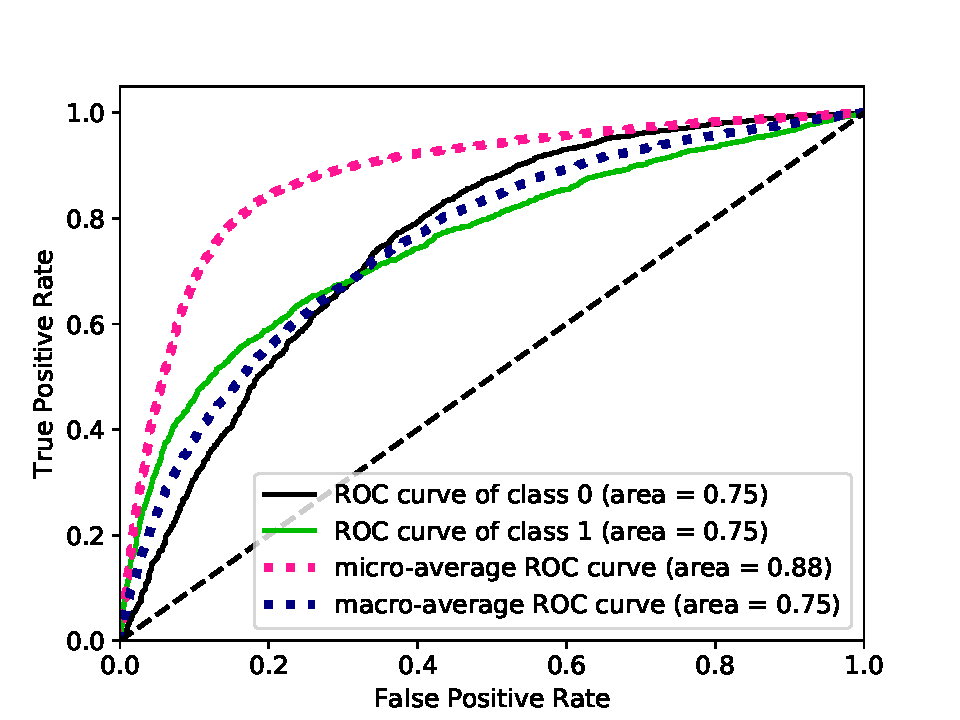
\includegraphics[width=0.75\textwidth]{ROC_Logreg_50e_100b_GD.pdf}    \caption[short]{Logistic regression gradient descent with 10000 iterations.}
% \end{subfigure}%
% \begin{subfigure}{.5\textwidth}
%     \centering
%     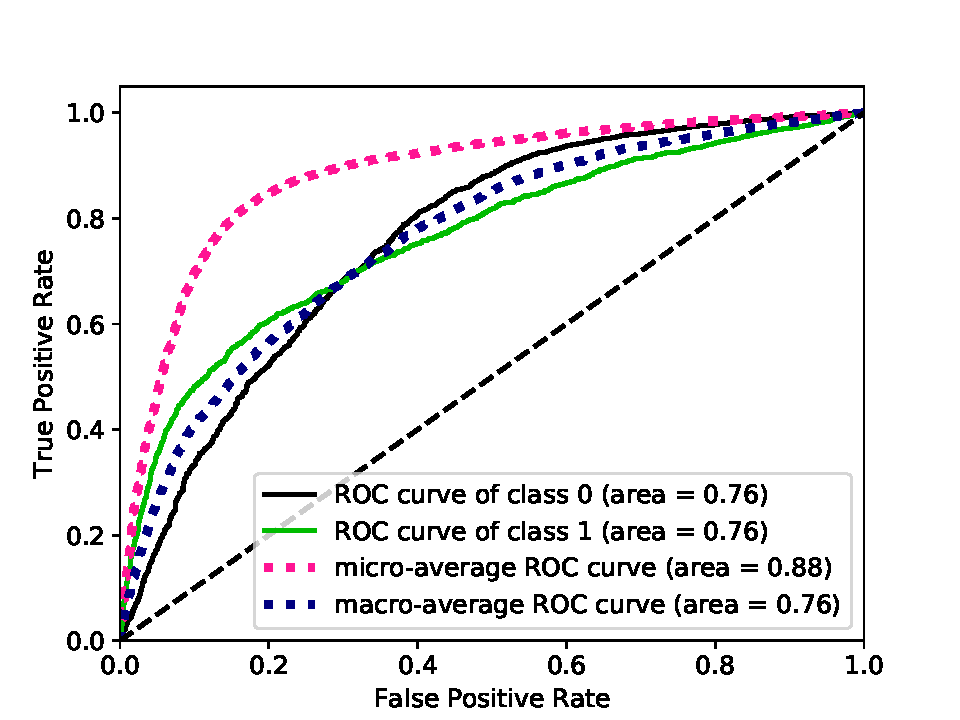
\includegraphics[width=0.75\textwidth]{ROC_Logreg_50e_100b_SGD.pdf}
%     \caption[short]{Logistic regression with stochastic gradient descent with 50 epochs and 100 mini batch size.}
% \end{subfigure}
% \begin{subfigure}{.5\textwidth}
%     \centering
%     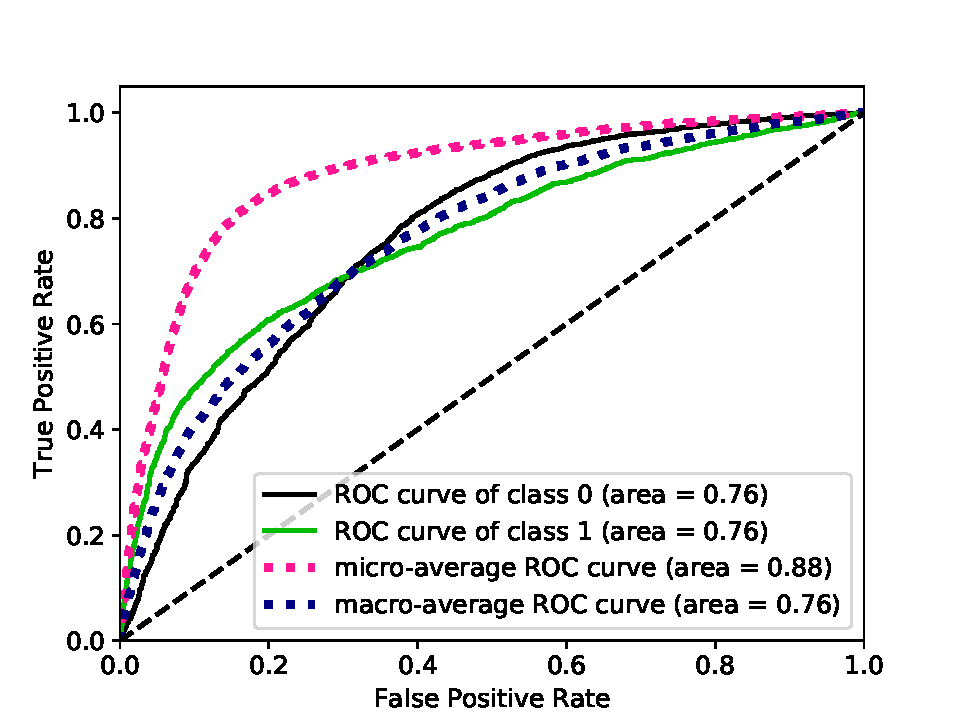
\includegraphics[width=0.75\textwidth]{ROC_Logreg_50e_100b_Sklearn.pdf}
%     \caption[short]{Logistic regression with scikit-learn.}
% \end{subfigure}%
% \begin{subfigure}{.5\textwidth}
%     \centering
%     \includegraphics[width=0.75\textwidth]{roc_20e_100b_64_32_16_sigsigsigsig.pdf}
%     \caption[short]{Neural network with 50 epochs, 100 mini batch size, three hidden layers of 64, 32 and 16 neurons. Sigmoid activation functions for hidden and output layers.}
% \end{subfigure}
% \centering\caption[short]{ROC curves for credit card default data.}
% \label{fig:roc_curves}
% \end{figure*}

% \begin{figure*}[t]
% \centering
% \begin{subfigure}{.5\textwidth}
%     \centering
%     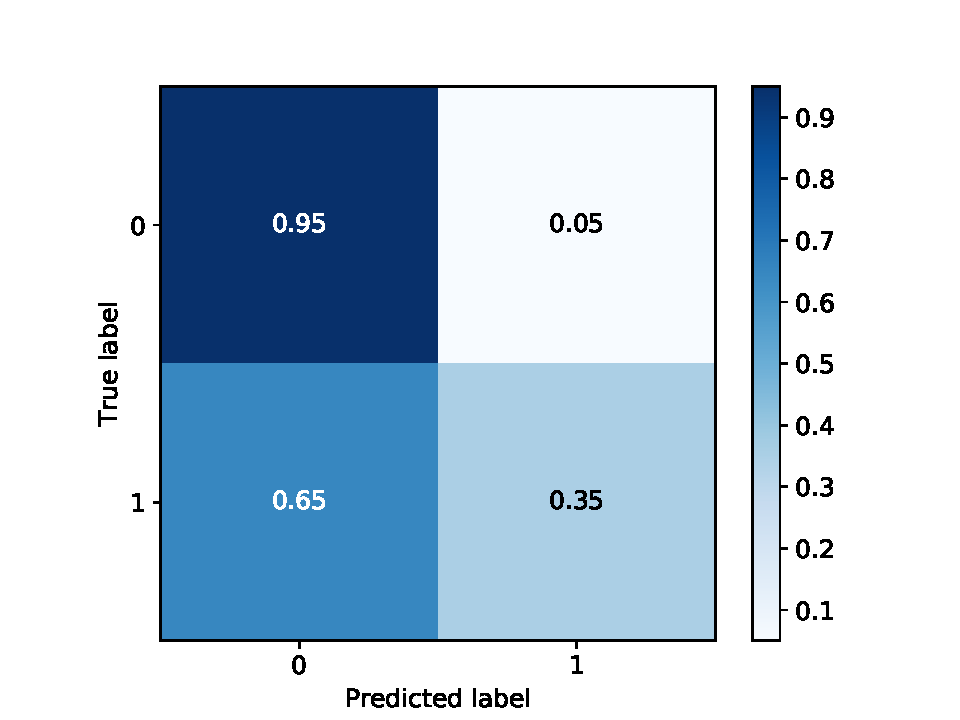
\includegraphics[width=0.75\textwidth]{conf_Logreg_50e_100b_GD.pdf}    \caption[short]{Logistic regression with gradient descent with 10000 iterations.}
% \end{subfigure}%
% \begin{subfigure}{.5\textwidth}
%     \centering
%     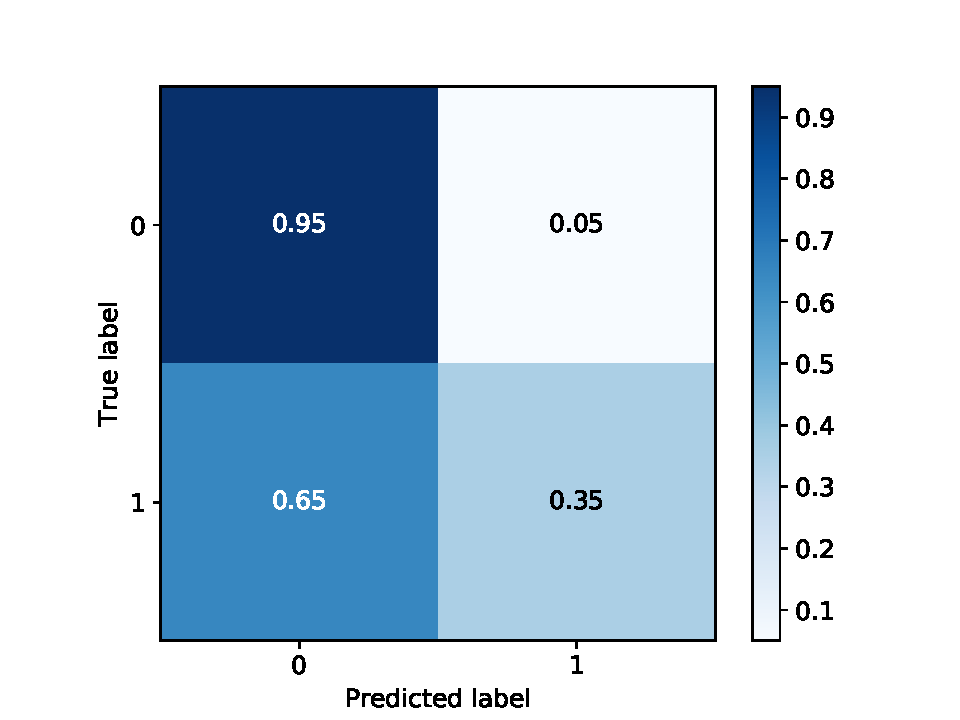
\includegraphics[width=0.75\textwidth]{conf_Logreg_50e_100b_SGD.pdf}
%     \caption[short]{Logistic regression with stochastic gradient descent with 50 epochs and 100 mini batch size.}
% \end{subfigure}
% \begin{subfigure}{.5\textwidth}
%     \centering
%     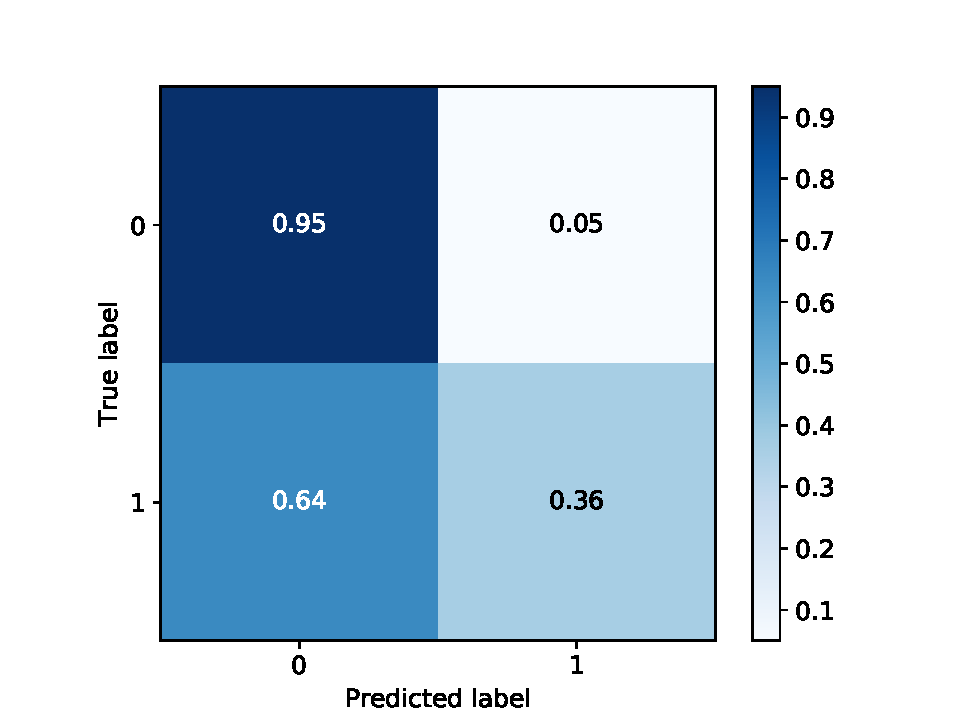
\includegraphics[width=0.75\textwidth]{conf_Logreg_50e_100b_Sklearn.pdf}
%     \caption[short]{Logistic regression with scikit learn.}
% \end{subfigure}%
% \begin{subfigure}{.5\textwidth}
%     \centering
%     \includegraphics[width=0.75\textwidth]{conf_20e_100b_64_32_16_sigsigsigsig.pdf}
%     \caption[short]{Neural network with 50 epochs, 100 mini batch size, three hidden layers of 64, 32 and 16 neurons. Sigmoid activation function for hidden and output layers.}
% \end{subfigure}
% \centering\caption[short]{Normalized confusion matrix on credit card default data.}
% \label{fig:norm_conf_mat}
% \end{figure*}


% \begin{figure*}[t]
% \centering
% \begin{subfigure}{.5\textwidth}
%     \centering
%     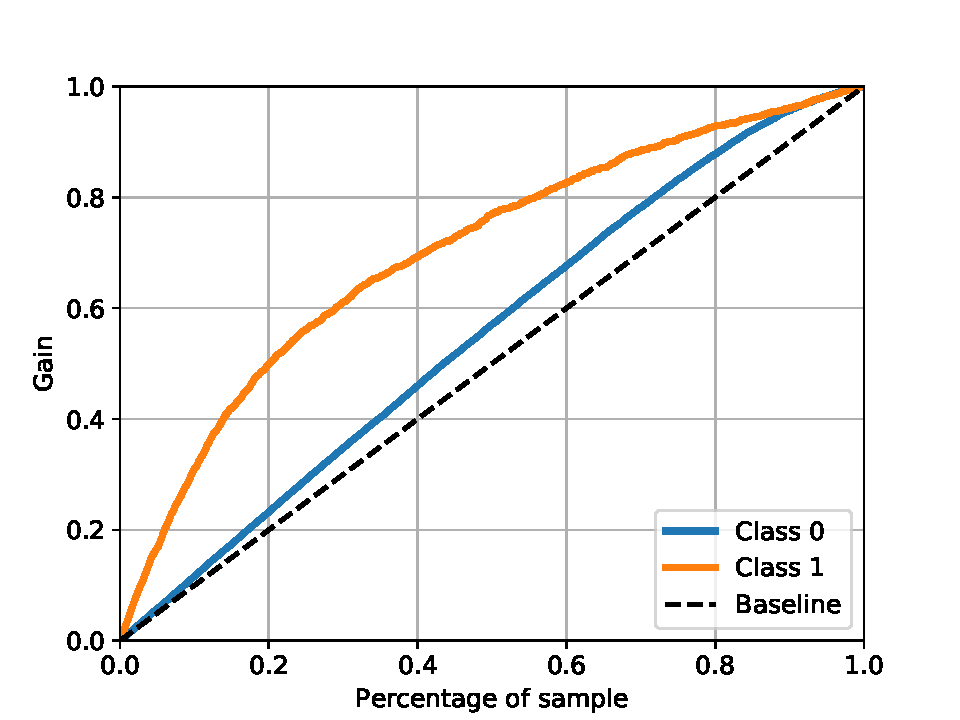
\includegraphics[width=0.75\textwidth]{gain_Logreg_50e_100b_GD.pdf}    \caption[short]{Logistic regression with gradient descent with 10000 iterations.}
% \end{subfigure}%
% \begin{subfigure}{.5\textwidth}
%     \centering
%     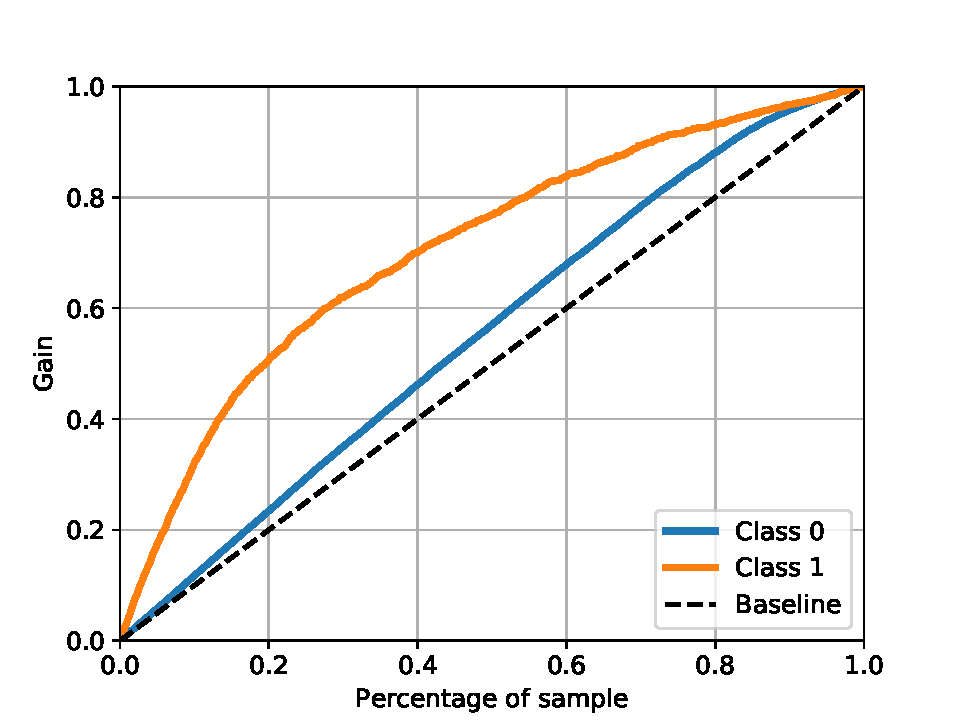
\includegraphics[width=0.75\textwidth]{gain_Logreg_50e_100b_SGD.pdf}
%     \caption[short]{Logistic regression with stochastic gradient descent with 50 epochs and 100 mini batch size.}
% \end{subfigure}
% \begin{subfigure}{.5\textwidth}
%     \centering
%     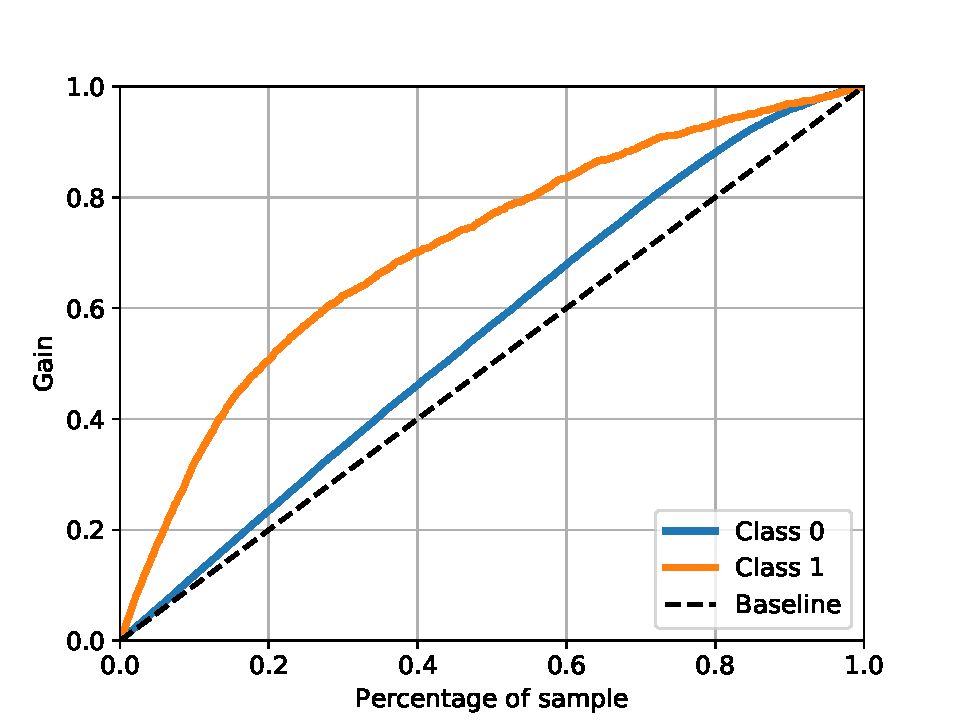
\includegraphics[width=0.75\textwidth]{gain_Logreg_50e_100b_Sklearn.pdf}
%     \caption[short]{Logistic regression with scikit-learn.}
% \end{subfigure}%
% \begin{subfigure}{.5\textwidth}
%     \centering
%     \includegraphics[width=0.75\textwidth]{gain_20e_100b_64_32_16_sigsigsigsig.pdf}
%     \caption[short]{Neural network with 20 epochs, 100 mini batch size, three hidden layers of 64, 32 and 16 neurons. Sigmoid activation function for hidden and output layers.}
% \end{subfigure}
% \centering\caption[short]{Cumulative gain for logistic regression on credit card default data.}
% \label{fig:cum_gain}
% \end{figure*}


\begin{figure}[b]
\subfloat{%
  \includegraphics[clip,width=\columnwidth]{gain_20e_100b_64_32_16_sigsigsigsig.pdf}%
  \subcaption{Own NN with 50 epochs and batch size 100.}
}
\subfloat{%
  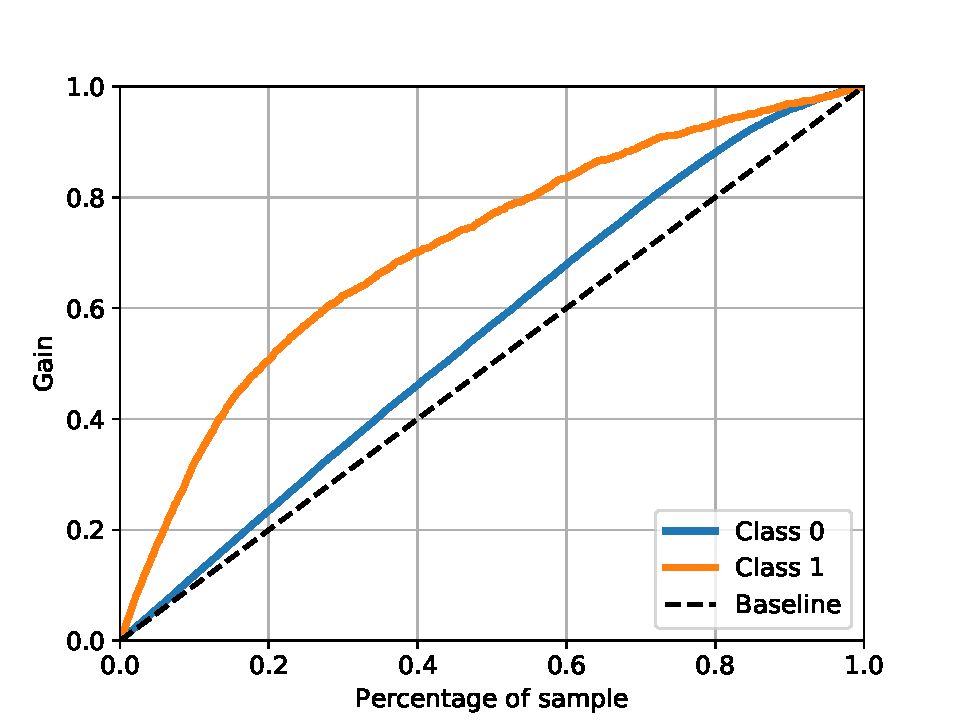
\includegraphics[clip,width=\columnwidth]{gain_Logreg_50e_100b_Sklearn.pdf}%
  \subcaption{Scikit-learn MLPClassifier neural network.}
}
\caption{Cumulative gain chart for credit card default data. Three hidden layers of 64, 32 and 16 neurons. Sigmoid activation function for hidden and output layers.}
\label{fig:cum_gain_NN}
\end{figure}

\begin{figure}[h!]
\subfloat{
  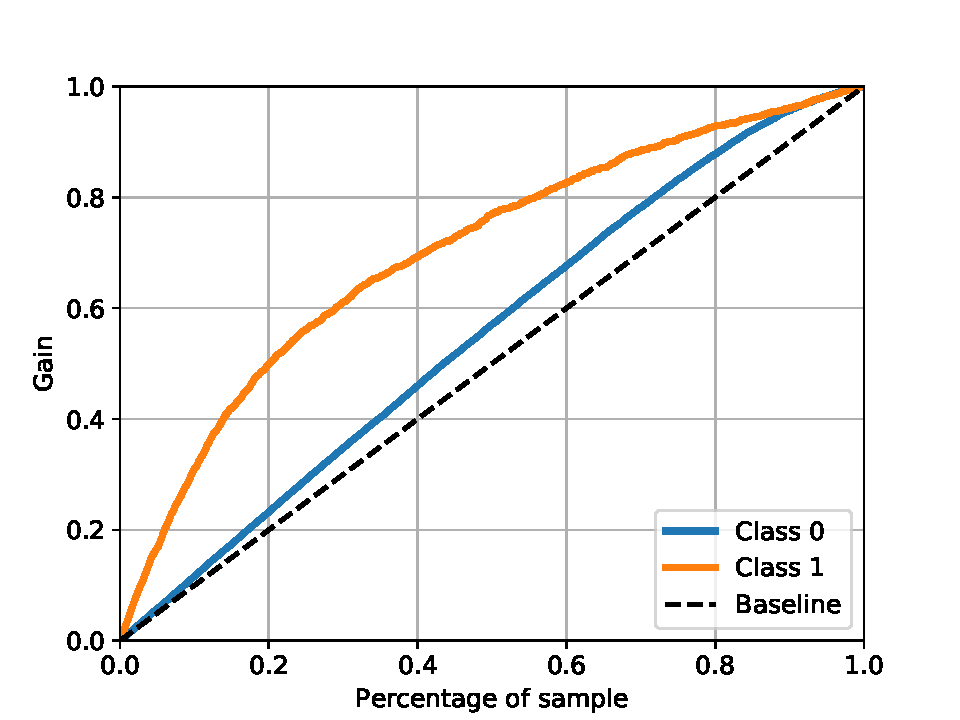
\includegraphics[clip,width=\columnwidth]{gain_Logreg_50e_100b_GD.pdf}
  \subcaption{Gradient descent with 10000 iterations.}
}
\subfloat{
  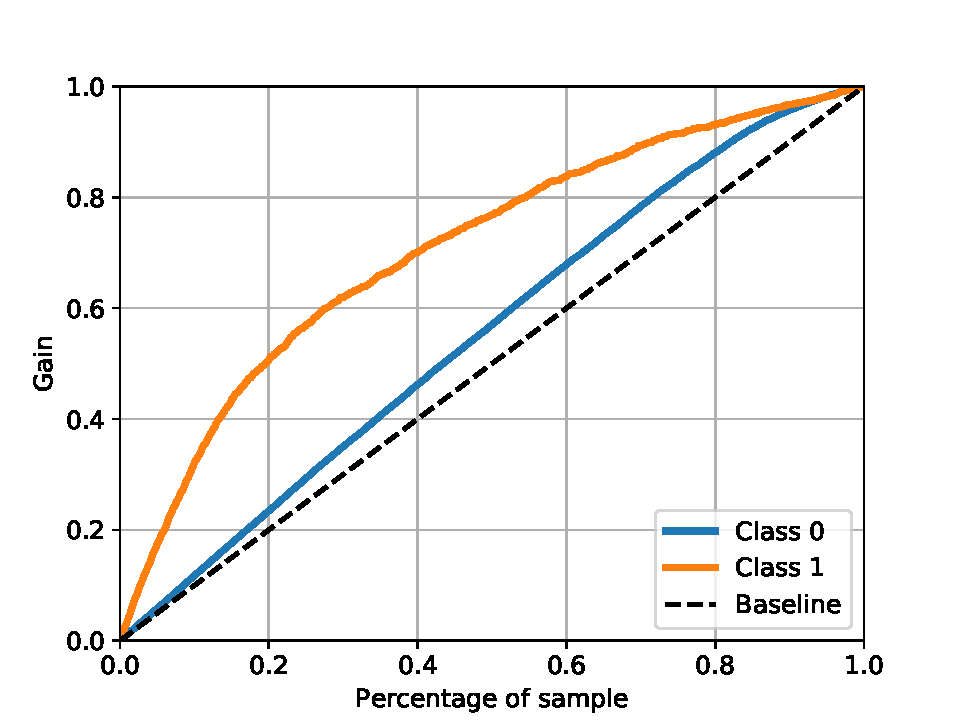
\includegraphics[clip,width=\columnwidth]{gain_Logreg_50e_100b_SGD.pdf}
  \subcaption{Stochastic gradient descent with 50 epochs and 100 mini batch size.}
}
\subfloat{
  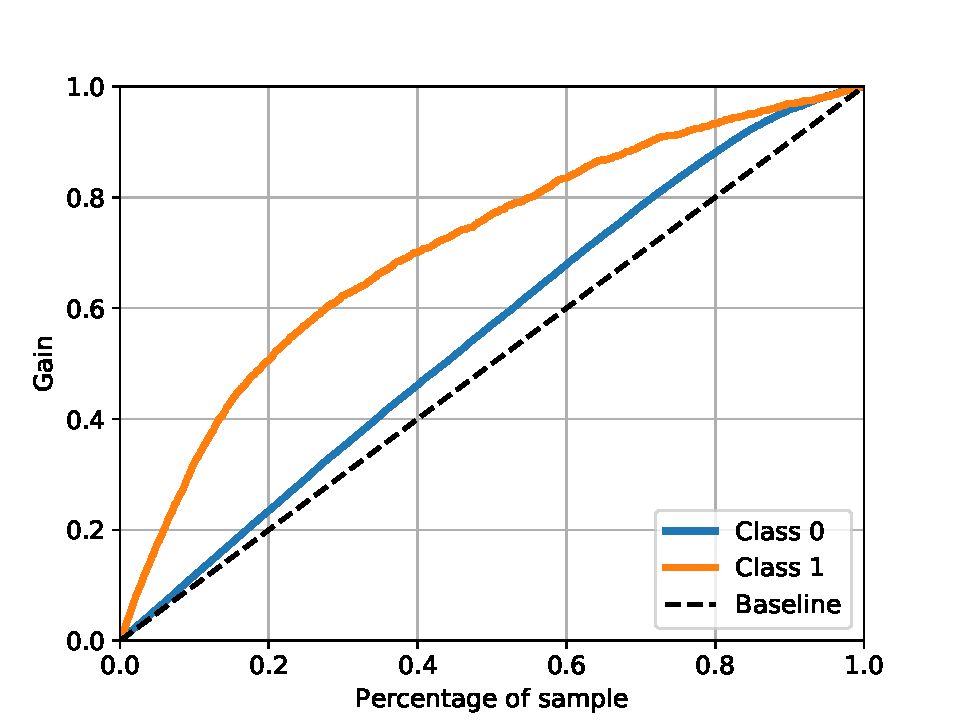
\includegraphics[clip,width=\columnwidth]{gain_Logreg_50e_100b_Sklearn.pdf}
  \subcaption{Scikit-learn.}
}
\caption{Cumulative gain chart for credit card default data, using different types of logistic regression.}
\label{fig:cum_gain_logreg}
\end{figure}

\begin{table}[b]
\caption{\label{tab:best_p_franke}%
Best polynomial degree and hyperparameter using Franke dataset for each model. A 50x50 grid with no added noise was used.
}
\begin{ruledtabular}
\begin{tabular}{lccr}
\textrm{}&
\multicolumn{1}{c}{\textrm{OLS}}&
\multicolumn{1}{c}{\textrm{Ridge}}&
\textrm{Lasso}\\
\colrule
Degree & 40 & 36 & 5 \\
Hyperparameter & N/A & $10^{-11}$ & $10^{-8}$ \\
MSE & $1.4 \cdot 10^{-5}$ & $1.0 \cdot 10^{-5}$ & $7.8 \cdot 10^{-3}$  \\
$R^2$ & 0.9998 & 0.9999 & 0.9222 \\
\end{tabular}
\end{ruledtabular}
\end{table}


\section{Discussion}\label{sec:discussion}

\subsection{Classification}
Because of the dependence on hyperparameters, neural networks often require many different test configurations. This is done by setting up a grid search, which means training a model for each combination of chosen hyperparameters. We decide the best model by evaluating the ROC score (ROC AUC (area under curve)) for each model, with respect to the hyperparameters. The reason for choosing ROC as a decider for the best model is that it takes true and false positives/negatives into account, while the accuracy score, comparing the prediction and the target, does not. The ROC AUC tells us how good the model is at distinguishing those who default and those who do not. The closer the AUC is to 1, the less false negatives and positives there are. An AUC of 0.5 would mean the model is randomly guessing between defaulting or not, as it cannot distinguish between them. The best ROC AUC for credit card case is $0.77$ by our neural network, with a corresponding test accuracy of $0.83$. The ROC AUC tells us that our model has a $77\%$ chance to correctly classify default or not.

Reviewing the confusion matrices (Fig. \ref{fig:conf_matrices_logreg} and \ref{fig:conf_matrices_NN}) of the different methods we can see that all models had most misclassification in cases where the customer defaulted. The bias in our data makes it easier for our model to not predict default, which makes it hard for the model to correctly classify the customers who default. Varied data will make it hard to create a reasonable model because recreating the noise of the data will result in low predictive power in the model. Likewise if a model can find some traits in the data that is possible to generalize it will still misclassify outliers and noise.

From Fig. \ref{fig:roc_curves_logreg} and \ref{fig:roc_curves_NN} we see that the methods yield similar results on the credit card dataset. The neural network performs better than logistic regression for both GD, SGD and scikit-learn's method. For logistic regression the best ROC score yields the same as for the logistic regression in scikit-learn. Comparing our neural network with the one found in scikit-learn, our neural network performed markedly better. Scikit-learn's MLPRegressor was outperformed by our neural, as well as all the methods for logistic regression. This could be the result of the scikit-learn neural network being more general and not tuned to our purpose like our own neural network and logistic regressions.

In Fig. \ref{fig:cum_gain_NN} and \ref{fig:cum_gain_logreg} we see that all methods yield similar results. The neural network has a slightly better gain curve for both classes. Logistic regression with GD again performs the worst and logistic regression with SGD and scikit-learn's logistic regression performs about equal. The gain charts show that the models perform approximately the same in terms of how effective they are at classifying.


\subsection{Regression}
From table \ref{tab:best_p_franke} we see that both OLS and ridge regression perform exceedingly well on the Franke dataset with no added noise. The $R^2$ scores are very close to 1 and the MSEs are both very low, on the order $10^{-5}$. Using a neural network on the same problem yields good results as well (Fig. \ref{fig:mse_r2_NN}), both in terms of $R^2$ score and MSE. A learning rate of $\eta =  0.0001$ and penalty $\lambda \leq 0.1$ gives the best-fitted neural networks. However, the performance is still not as good as traditional regression methods, though it does perform better than lasso regression in this case.

\section{Conclusions}
We classified the credit card data using both our own and scikit-learn's methods for logistic regression and neural networks to classify defaulting and not defaulting credit card customers. Our own neural network performed overall a little better than the logistic regressions methods. It also performed significantly better than scikit-learn's neural network with AUC of $0.77$ compared to $0.68$. This may have been because of the more generalized methods employed by scikit-learn, and the fact that the dataset has few correlations to predict default. A possible way to improve performance in the future would be using a principal component analysis (PCA), to reduce the dimensionality of the credit card data.

For regression on the Franke dataset, our neural network did not perform better than ordinary least squares or ridge regression. Even though the neural network had a more complex structure than the traditional regression models, the network did not pick up on the trend as easily as a model built on polynomials.

The reason for this may be that the features per sample in our NN are just the $x$ and $y$ coordinates of a height $z$, so that each individual sample is treated independent of the other samples. This means that the structure of the neural network does not assume any connections between the different coordinates. It is possible that a convolutional neural network would be better suited for this, as this type of neural net would be able to take the entire grid of $x$ and $y$ as a single input.

When reviewing the overall performance of our methods we can conclude that neural networks are well suited for many different problems. While they are dependent on many hyperparameters they can often give results comparable to or even better than other methods.


%\onecolumngrid
\appendix
\section{Appendix}
In Fig. \ref{fig:train_acc} we can see that the neural network does not overfit, the value does not stray far from the observed test accuracy.
\begin{figure}[b]
\includegraphics[width=\columnwidth]{trainacc_20e_100b_64_32_16_sigsigsigsig.pdf}
\caption{\label{fig:train_acc} Training accuracy for neural network on credit card default data. 50 epochs, 100 mini batch size, two hidden layers of 64, 32 and 16 neurons. Sigmoid activation functions for hidden and output layers.}
\end{figure}

% \begin{figure}[b]
% \includegraphics{data1_cho}% Here is how to import EPS art
% \caption{\label{fig:epsart} A figure caption. The figure captions are
% automatically numbered.}
% \end{figure}

% \begin{figure*}
% \includegraphics{fig_2}% Here is how to import EPS art
% \caption{\label{fig:wide}Use the figure* environment to get a wide
% figure that spans the page in \texttt{twocolumn} formatting.}
% \end{figure*}


% \begin{table*}
% \caption{\label{tab:table3}This is a wide table that spans the full page
% width in a two-column layout. It is formatted using the
% \texttt{table*} environment. It also demonstates the use of
% \textbackslash\texttt{multicolumn} in rows with entries that span
% more than one column.}
% \begin{ruledtabular}
% \begin{tabular}{ccccc}
%  &\multicolumn{2}{c}{$D_{4h}^1$}&\multicolumn{2}{c}{$D_{4h}^5$}\\
%  Ion&1st alternative&2nd alternative&lst alternative
% &2nd alternative\\ \hline
%  K&$(2e)+(2f)$&$(4i)$ &$(2c)+(2d)$&$(4f)$ \\
%  Mn&$(2g)$\footnote{The $z$ parameter of these positions is $z\sim\frac{1}{4}$.}
%  &$(a)+(b)+(c)+(d)$&$(4e)$&$(2a)+(2b)$\\
%  Cl&$(a)+(b)+(c)+(d)$&$(2g)$\footnotemark[1]
%  &$(4e)^{\text{a}}$\\
%  He&$(8r)^{\text{a}}$&$(4j)^{\text{a}}$&$(4g)^{\text{a}}$\\
%  Ag& &$(4k)^{\text{a}}$& &$(4h)^{\text{a}}$\\
% \end{tabular}
% \end{ruledtabular}
% \end{table*}

% \begin{table}[b]
% \caption{\label{tab:table4}%
% Numbers in columns Three--Five are aligned with the ``d'' column specifier
% (requires the \texttt{dcolumn} package).
% Non-numeric entries (those entries without a ``.'') in a ``d'' column are aligned on the decimal point.
% Use the ``D'' specifier for more complex layouts. }
% \begin{ruledtabular}
% \begin{tabular}{ccddd}
% One&Two&
% \multicolumn{1}{c}{\textrm{Three}}&
% \multicolumn{1}{c}{\textrm{Four}}&
% \multicolumn{1}{c}{\textrm{Five}}\\
% %\mbox{Three}&\mbox{Four}&\mbox{Five}\\
% \hline
% one&two&\mbox{three}&\mbox{four}&\mbox{five}\\
% He&2& 2.77234 & 45672. & 0.69 \\
% C\footnote{Some tables require footnotes.}
%   &C\footnote{Some tables need more than one footnote.}
%   & 12537.64 & 37.66345 & 86.37 \\
% \end{tabular}
% \end{ruledtabular}
% \end{table}


% Tables~\ref{tab:table1}, \ref{tab:table3}, \ref{tab:table4}, and \ref{tab:table2}%
% \begin{table}[b]
% \caption{\label{tab:table2}
% A table with numerous columns that still fits into a single column.
% Here, several entries share the same footnote.
% Inspect the \LaTeX\ input for this table to see exactly how it is done.}
% \begin{ruledtabular}
% \begin{tabular}{cccccccc}
%  &$r_c$ (\AA)&$r_0$ (\AA)&$\kappa r_0$&
%  &$r_c$ (\AA) &$r_0$ (\AA)&$\kappa r_0$\\
% \hline
% Cu& 0.800 & 14.10 & 2.550 &Sn\footnotemark[1]
% & 0.680 & 1.870 & 3.700 \\
% Ag& 0.990 & 15.90 & 2.710 &Pb\footnotemark[2]
% & 0.450 & 1.930 & 3.760 \\
% Au& 1.150 & 15.90 & 2.710 &Ca\footnotemark[3]
% & 0.750 & 2.170 & 3.560 \\
% Mg& 0.490 & 17.60 & 3.200 &Sr\footnotemark[4]
% & 0.900 & 2.370 & 3.720 \\
% Zn& 0.300 & 15.20 & 2.970 &Li\footnotemark[2]
% & 0.380 & 1.730 & 2.830 \\
% Cd& 0.530 & 17.10 & 3.160 &Na\footnotemark[5]
% & 0.760 & 2.110 & 3.120 \\
% Hg& 0.550 & 17.80 & 3.220 &K\footnotemark[5]
% &  1.120 & 2.620 & 3.480 \\
% Al& 0.230 & 15.80 & 3.240 &Rb\footnotemark[3]
% & 1.330 & 2.800 & 3.590 \\
% Ga& 0.310 & 16.70 & 3.330 &Cs\footnotemark[4]
% & 1.420 & 3.030 & 3.740 \\
% In& 0.460 & 18.40 & 3.500 &Ba\footnotemark[5]
% & 0.960 & 2.460 & 3.780 \\
% Tl& 0.480 & 18.90 & 3.550 & & & & \\
% \end{tabular}
% \end{ruledtabular}
% \footnotetext[1]{Here's the first, from Ref.~\onlinecite{feyn54}.}
% \footnotetext[2]{Here's the second.}
% \footnotetext[3]{Here's the third.}
% \footnotetext[4]{Here's the fourth.}
% \footnotetext[5]{And etc.}
% \end{table}

% \begin{acknowledgments}

% \end{acknowledgments}

% \appendix

% \section{Appendixes}

% The \nocite command causes all entries in a bibliography to be printed out
% whether or not they are actually referenced in the text. This is appropriate
% for the sample file to show the different styles of references, but authors
% most likely will not want to use it.
\nocite{*}

\bibliography{main}% Produces the bibliography via BibTeX.

\end{document}
%
% ****** End of file apssamp.tex ******
